\subsection*{Fixed by the helper}
These needed a word the old brain had never seen. The helper knows what a bolt, a hull, a chestpiece and a headband look like.

\needspace{9\baselineskip}
\noindent\texttt{feather/battery-charging/1} \quad \emph{``Change the lightning bolt to red.''} \quad {\small\color{grey} 3 lines to choose from}\\[3pt]
\begin{center}
\begin{tabular}{@{}c@{\hspace{9mm}}c@{\hspace{9mm}}c@{}}

\includegraphics[width=2.6cm]{img/feather_battery-charging_1_gold.png} &

\includegraphics[width=2.6cm]{img/feather_battery-charging_1_base.png} &

\includegraphics[width=2.6cm]{img/feather_battery-charging_1_fused.png} \\
{\small Gold: \texttt{n3}} &
{\small Old brain: \texttt{n2} \textcolor{pink}{$\times$}} &
{\small Mix: \texttt{n3} \textcolor{blue}{\checkmark}} \\
\end{tabular}\\[-2pt]
{\small\color{grey} Mix's order: \texttt{n3 > n2 > n1} \quad count head said $k=1$}
\end{center}

\needspace{9\baselineskip}
\noindent\texttt{tabler/sailboat/1} \quad \emph{``Change the wavy water line to red.''} \quad {\small\color{grey} 4 lines to choose from}\\[3pt]
\begin{center}
\begin{tabular}{@{}c@{\hspace{9mm}}c@{\hspace{9mm}}c@{}}

\includegraphics[width=2.6cm]{img/tabler_sailboat_1_gold.png} &

\includegraphics[width=2.6cm]{img/tabler_sailboat_1_base.png} &

\includegraphics[width=2.6cm]{img/tabler_sailboat_1_fused.png} \\
{\small Gold: \texttt{n1}} &
{\small Old brain: \texttt{n3} \textcolor{pink}{$\times$}} &
{\small Mix: \texttt{n1} \textcolor{blue}{\checkmark}} \\
\end{tabular}\\[-2pt]
{\small\color{grey} Mix's order: \texttt{n1 > n2 > n4 > n3} \quad count head said $k=1$}
\end{center}

\needspace{9\baselineskip}
\noindent\texttt{tabler/stethoscope/2} \quad \emph{``Change the circular chestpiece to red.''} \quad {\small\color{grey} 5 lines to choose from}\\[3pt]
\begin{center}
\begin{tabular}{@{}c@{\hspace{9mm}}c@{\hspace{9mm}}c@{}}

\includegraphics[width=2.6cm]{img/tabler_stethoscope_2_gold.png} &

\includegraphics[width=2.6cm]{img/tabler_stethoscope_2_base.png} &

\includegraphics[width=2.6cm]{img/tabler_stethoscope_2_fused.png} \\
{\small Gold: \texttt{n5}} &
{\small Old brain: \texttt{n3} \textcolor{pink}{$\times$}} &
{\small Mix: \texttt{n5} \textcolor{blue}{\checkmark}} \\
\end{tabular}\\[-2pt]
{\small\color{grey} Mix's order: \texttt{n5 > n1 > n2 > n3 > n4} \quad count head said $k=1$}
\end{center}

\needspace{9\baselineskip}
\noindent\texttt{feather/headphones/2} \quad \emph{``Change the curved headband to red.''} \quad {\small\color{grey} 2 lines to choose from}\\[3pt]
\begin{center}
\begin{tabular}{@{}c@{\hspace{9mm}}c@{\hspace{9mm}}c@{}}

\includegraphics[width=2.6cm]{img/feather_headphones_2_gold.png} &

\includegraphics[width=2.6cm]{img/feather_headphones_2_base.png} &

\includegraphics[width=2.6cm]{img/feather_headphones_2_fused.png} \\
{\small Gold: \texttt{n1}} &
{\small Old brain: \texttt{n2} \textcolor{pink}{$\times$}} &
{\small Mix: \texttt{n1} \textcolor{blue}{\checkmark}} \\
\end{tabular}\\[-2pt]
{\small\color{grey} Mix's order: \texttt{n1 > n2} \quad count head said $k=1$}
\end{center}

\subsection*{Broken by the helper}
The old brain had these right. Both describe a tiny mark by where it is, and the three little pictures do not separate it from the arcs around it.

\needspace{9\baselineskip}
\noindent\texttt{feather/watch/1} \quad \emph{``Change the watch hands to red.''} \quad {\small\color{grey} 3 lines to choose from}\\[3pt]
\begin{center}
\begin{tabular}{@{}c@{\hspace{9mm}}c@{\hspace{9mm}}c@{}}

\includegraphics[width=2.6cm]{img/feather_watch_1_gold.png} &

\includegraphics[width=2.6cm]{img/feather_watch_1_base.png} &

\includegraphics[width=2.6cm]{img/feather_watch_1_fused.png} \\
{\small Gold: \texttt{n2}} &
{\small Old brain: \texttt{n2} \textcolor{blue}{\checkmark}} &
{\small Mix: \texttt{n3} \textcolor{pink}{$\times$}} \\
\end{tabular}\\[-2pt]
{\small\color{grey} Mix's order: \texttt{n3 > n2 > n1} \quad count head said $k=1$}
\end{center}

\needspace{9\baselineskip}
\noindent\texttt{feather/wifi/2} \quad \emph{``Change the small dot below the arcs to red.''} \quad {\small\color{grey} 4 lines to choose from}\\[3pt]
\begin{center}
\begin{tabular}{@{}c@{\hspace{9mm}}c@{\hspace{9mm}}c@{}}

\includegraphics[width=2.6cm]{img/feather_wifi_2_gold.png} &

\includegraphics[width=2.6cm]{img/feather_wifi_2_base.png} &

\includegraphics[width=2.6cm]{img/feather_wifi_2_fused.png} \\
{\small Gold: \texttt{n4}} &
{\small Old brain: \texttt{n4} \textcolor{blue}{\checkmark}} &
{\small Mix: \texttt{n2} \textcolor{pink}{$\times$}} \\
\end{tabular}\\[-2pt]
{\small\color{grey} Mix's order: \texttt{n2 > n4 > n3 > n1} \quad count head said $k=1$}
\end{center}

\subsection*{Right order, wrong count}
The mix puts every gold line first. Then the old count head takes too few (one) or too many (four).

\needspace{9\baselineskip}
\noindent\texttt{feather/save/1} \quad \emph{``Change the two interior panels of the floppy disk to red.''} \quad {\small\color{grey} 3 lines to choose from}\\[3pt]
\begin{center}
\begin{tabular}{@{}c@{\hspace{9mm}}c@{\hspace{9mm}}c@{}}

\includegraphics[width=2.6cm]{img/feather_save_1_gold.png} &

\includegraphics[width=2.6cm]{img/feather_save_1_base.png} &

\includegraphics[width=2.6cm]{img/feather_save_1_fused.png} \\
{\small Gold: \texttt{n2, n3}} &
{\small Old brain: \texttt{n2} \textcolor{pink}{$\times$}} &
{\small Mix: \texttt{n2} \textcolor{pink}{$\times$}} \\
\end{tabular}\\[-2pt]
{\small\color{grey} Mix's order: \texttt{n2 > n3 > n1} \quad count head said $k=1$}
\end{center}

\needspace{9\baselineskip}
\noindent\texttt{tabler/palette/1} \quad \emph{``Change all three circular paint wells to red.''} \quad {\small\color{grey} 4 lines to choose from}\\[3pt]
\begin{center}
\begin{tabular}{@{}c@{\hspace{9mm}}c@{\hspace{9mm}}c@{}}

\includegraphics[width=2.6cm]{img/tabler_palette_1_gold.png} &

\includegraphics[width=2.6cm]{img/tabler_palette_1_base.png} &

\includegraphics[width=2.6cm]{img/tabler_palette_1_fused.png} \\
{\small Gold: \texttt{n2, n3, n4}} &
{\small Old brain: \texttt{n4} \textcolor{pink}{$\times$}} &
{\small Mix: \texttt{n2} \textcolor{pink}{$\times$}} \\
\end{tabular}\\[-2pt]
{\small\color{grey} Mix's order: \texttt{n2 > n4 > n3 > n1} \quad count head said $k=1$}
\end{center}

\needspace{9\baselineskip}
\noindent\texttt{feather/truck/1} \quad \emph{``Change both truck wheels to red.''} \quad {\small\color{grey} 4 lines to choose from}\\[3pt]
\begin{center}
\begin{tabular}{@{}c@{\hspace{9mm}}c@{\hspace{9mm}}c@{}}
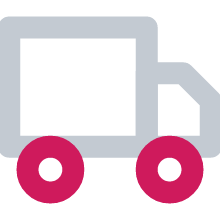
\includegraphics[width=2.6cm]{img/feather_truck_1_gold.png} &

\includegraphics[width=2.6cm]{img/feather_truck_1_base.png} &

\includegraphics[width=2.6cm]{img/feather_truck_1_fused.png} \\
{\small Gold: \texttt{n3, n4}} &
{\small Old brain: \texttt{n1, n2, n3, n4} \textcolor{pink}{$\times$}} &
{\small Mix: \texttt{n1, n2, n3, n4} \textcolor{pink}{$\times$}} \\
\end{tabular}\\[-2pt]
{\small\color{grey} Mix's order: \texttt{n4 > n3 > n1 > n2} \quad count head said $k=4$}
\end{center}

\subsection*{Still wrong}
Thin edges and outlines. When you highlight the edge, the picture looks almost the same as when you highlight the part next to it.

\needspace{9\baselineskip}
\noindent\texttt{feather/bell/2} \quad \emph{``Change the clapper below the bell to red.''} \quad {\small\color{grey} 2 lines to choose from}\\[3pt]
\begin{center}
\begin{tabular}{@{}c@{\hspace{9mm}}c@{\hspace{9mm}}c@{}}

\includegraphics[width=2.6cm]{img/feather_bell_2_gold.png} &

\includegraphics[width=2.6cm]{img/feather_bell_2_base.png} &

\includegraphics[width=2.6cm]{img/feather_bell_2_fused.png} \\
{\small Gold: \texttt{n2}} &
{\small Old brain: \texttt{n1} \textcolor{pink}{$\times$}} &
{\small Mix: \texttt{n1} \textcolor{pink}{$\times$}} \\
\end{tabular}\\[-2pt]
{\small\color{grey} Mix's order: \texttt{n1 > n2} \quad count head said $k=1$}
\end{center}

\needspace{9\baselineskip}
\noindent\texttt{tabler/flask/1} \quad \emph{``Change the horizontal lip at the very top to red.''} \quad {\small\color{grey} 3 lines to choose from}\\[3pt]
\begin{center}
\begin{tabular}{@{}c@{\hspace{9mm}}c@{\hspace{9mm}}c@{}}

\includegraphics[width=2.6cm]{img/tabler_flask_1_gold.png} &

\includegraphics[width=2.6cm]{img/tabler_flask_1_base.png} &

\includegraphics[width=2.6cm]{img/tabler_flask_1_fused.png} \\
{\small Gold: \texttt{n1}} &
{\small Old brain: \texttt{n3} \textcolor{pink}{$\times$}} &
{\small Mix: \texttt{n3} \textcolor{pink}{$\times$}} \\
\end{tabular}\\[-2pt]
{\small\color{grey} Mix's order: \texttt{n3 > n1 > n2} \quad count head said $k=1$}
\end{center}
